\documentclass[10pt,a4paper]{article}


\usepackage[protrusion=true,expansion=true]{microtype} % Better typography
\usepackage[colorlinks=true, allcolors=black]{hyperref}
\usepackage{graphicx} % Required for including pictures
\graphicspath{ {images/} }
\usepackage{wrapfig} % Allows in-line images
\usepackage{natbib}

\usepackage[table]{xcolor}
\definecolor{tableRed}{rgb}{1.0, 0.5, 0.5}
\definecolor{tableGreen}{rgb}{0.5, 1.0, 0.5}

\usepackage[section]{placeins}




\usepackage[english]{babel}
\usepackage[utf8]{inputenc}
\usepackage{fullpage}
\usepackage{amsmath}

\usepackage[toc,page]{appendix}

\usepackage[colorinlistoftodos]{todonotes}

\usepackage{amssymb}

\usepackage{pdflscape}

\newcommand{\plogo}{\fbox{$\mathcal{PL}$}} % Generic dummy publisher logo



\title{Natalis Business Plan}
\author{William Kennerley\\
Ben Plumley\\
Max Sandberg\\
Oliver Gray\\
Caroline Moir\\
Darien Opperman}
\date{\today}

\begin{document}

\begin{titlepage} % Suppresses headers and footers on the title page

	\centering % Centre everything on the title page

	\scshape % Use small caps for all text on the title page

	\vspace*{\baselineskip} % White space at the top of the page

	%------------------------------------------------
	%	Title
	%------------------------------------------------



	\vspace{0.75\baselineskip} % Whitespace above the title

	{\Huge Natalis Business Plan} % Title

	\vspace{0.75\baselineskip} % Whitespace below the title



	\vspace{2\baselineskip} % Whitespace after the title block

	
\includegraphics[width=\linewidth/2]{logo.png}

		\vspace{3\baselineskip} % Whitespace after the title block

	%------------------------------------------------
	%	Subtitle
	%------------------------------------------------

For the consumer who has the need to show loved ones they care, Natalis is a greetings card subscription service which offers a wide range of high-quality, hand made cards. Unlike existing offerings, Natalis reminds the customer when special dates draw close and provides them with everything they need to send a sentimental message.

	\vspace*{3\baselineskip} % Whitespace under the subtitle

	%------------------------------------------------
	%	Editor(s)
	%------------------------------------------------


	\vspace{0.5\baselineskip} % Whitespace before the editors

	 % Editor list
{\scshape\Large Oliver Gray\\ }
{\scshape\Large William Kennerley\\}
{\scshape\Large Caroline Moir\\}
{\scshape\Large Darien Opperman\\ }
{\scshape\Large Ben Plumley\\}
{\scshape\Large Max Sandberg\\}



	\vspace{1.0\baselineskip} % Whitespace below the editor list


	\vfill % Whitespace between editor names and publisher logo

	%------------------------------------------------
	%	Publisher
	%------------------------------------------------


	\vspace{0.3\baselineskip} % Whitespace under the publisher logo

	\today


\end{titlepage}


\raggedright
\setlength{\parskip}{6pt}
\setlength{\parindent}{0pt}
% \maketitle

\section*{Our Product}
\subsection*{The Problem}
Consumers across the UK send and receive greetings cards to demonstrate their love and respect for their friends and family. Consumers engage in this practice because of their needs for social belonging and esteem. In particular, greetings cards are chosen to fulfil these needs as they bear substantial conditional and emotional value; two values which consumers require a product provide to fulfil their purpose in demonstrating love and respect. However, in the current market, the choice available to the consumer is tightly constrained by the functional and social needs that they have of the product, limiting them to just a few options.

\subsection*{Consumer Needs}
The greetings card market aims to satisfy the following six consumer needs and values. These needs and values are drawn from the fundamental works by \citet{maslow1943theory} and \citet{sheth1991we}:
\begin{enumerate}
  \item Social belonging theorises that all humans have a desire to be part of social groups of all sizes, and have an innate need to love and feel loved by others. Since their invention, greetings cards have been a popular method to demonstrate one's feelings for another person on meaningful occasions, such as birthdays, religious holidays and family milestones. By sending a greetings card, the sender demonstrates their love for another person, and in return, the recipient will feel loved upon reading it.
  \item Emotional values represent the emotional feeling which the consumer will receive from the product. With greetings cards, the full emotional value is only realised when it has been received. The demonstration of love which greetings cards provide exemplify their value.
  \item Esteem is the need for a high-evaluation of one's self. Typically, this need is fulfilled through self-esteem, respect for others or respect by others. Greetings cards demonstrate the respect the sender has for the recipient: by showing the recipient that their important day is important to the sender too. Furthermore, upon receiving a greetings card, the recipient gains a boost to their self-esteem.
  \item Functional values are a traditional driver of consumer choice. The functional values in the chosen problem space, described above, include: the choice of designs of greetings cards available for purchase, the price of the cards and the time it will take the consumer to complete their customer journey \citep{edelman2015competing}. The customer journey of a conventional greetings card starts by visiting the store, followed by writing the card, then visiting the post office and finally getting the card in the hands of the recipient. A product with high functional value, such as a card with a more attractive design or a card from a shop which is closer, is more likely to be purchased by the consumer. The Natalis customer journey aims offer far greater functional value to customers than what is offered by a traditional greetings card.
  \item Social values are the values gained from a purchase that leads to a sense of belonging to a community. While there is no specific social group or tribe \citep{canniford2011manage} associated with greetings cards, the quality and style of the card, as well as the message that is written on the card, can convey a lot about the social standing of the consumer and the tribes with which they associate. The card with the highest social value to the consumer, the one they purchase, is the card which best aligns with their self-image in terms of design and message.
  \item Conditional values are temporary values which are related to a specific set of circumstances associated with the object the consumer is looking to purchase. By their nature, greetings cards have a strong conditional value as they focus on commemorating a single event. The conditional value of greetings cards increases as a result of two factors: the uniqueness of the event and the closer to the date the card is purchased and received. All cards offered by Natalis will have a high conditional value as a result of our business model.
\end{enumerate}

\subsection*{Value Proposition}
Natalis is a web-based subscription service for greetings cards.

Customers enter significant dates relating to each contact, such as birthdays and anniversaries, and are offered a selection of appropriate greetings cards close to the entered dates. Their card of choice will be mailed to them along with a stamped envelope addressed to their recipient. The customer simply writes the inside of the card and posts it when convenient in their nearest postbox. The customer is spared the hassle of visiting their high-street card shop and post office, allowing them to focus on the sentiment.

Users interact with Natalis through our website. Creating an account is required so we can store their contacts' information. Upon account creation, users are prompted to add a contact; the information required for their contact is the important date and event type, so appropriate card options can be offered at a suitable time, and their address, so the stamped envelope can be prepared. Each contact will also have a subscription type: repeating or single. Once the contact is created, they can leave the rest to us.

Two weeks before the chosen date, the customer is emailed a selection of cards which we think they might like, along with a link to the website where they can view the full range of designs. The selected design is then packaged with a stamped envelope, printed with their recipient's address and dispatched to the customer as quickly as possible. Upon receipt of the card, the customer can take the time to fill out a meaningful message inside the card, place it inside the included envelope and post it at their convenience.

There are many mass-produced, generic cards available on the high-street and online. The aim of Natalis is to provide a similar accessibility level for high quality, premium cards. On top of being able to access quality greetings cards, customers also gain the convenience of having the choice of cards emailed to them on a set-and-forget schedule, making the disaster situation of forgetting a birthday or anniversary less of a concern for the customer.

\subsubsection*{Meeting the Customer Needs}
The value proposition of Natalis fulfils the six needs described above.

The need for social belonging is met when customers reach the enjoyment phase of their customer journey \citep{edelman2015competing}: once the intended recipient has received their card and the display of affection within. Natalis provides a mechanism which allows greetings cards to be sent more easily, facilitating customers in fulfilling their social belonging need.


Natalis fulfils the customer's emotional values by offering greetings cards which serve as a symbol of sentiment from the sender. This helps the customer feel accomplished knowing that they have surpasssed the expectations of their recipient. This positive feeling is also mirrored by the recipient of the card, who feels desired and loved, understanding that the sender put effort into them.

The need for esteem is fulfilled through the customer's display of love and respect for the recipient, which is embodied by the greetings cards distributed by Natalis. For the recipient, the emotional experience of feeling loved and valued helps to build their esteem. If consumers forget important dates, they risk their self-esteem. Natalis mitigates this risk to self-esteem through email reminders which are triggered when important dates draw closer.

Natalis meets the functional values of the consumer through two channels. Firstly, the total time taken to complete their customer journey is shortened; most respondents in our market validation surveys visit high-street card shops to buy greetings cards. Not only does Natalis offer a selection of cards over the internet, removing the time taken to travel to high-street shop, it also provides a pre-selected, recommended list of cards to the customer in the email notification they receive, which will reduce the time taken to choose a card. additionally, the included stamped envelope eliminates the time that would be spent queueing at the post office to send their card. Secondly, Natalis will offer a wide variety of high-quality card designs which can't be found in high-street shops; the wide range of unique designs adds to the functional value of the cards.

Similarly, the wide range of card designs can fulfil the social values of the customer. This is because, the customer can pick a card design which they believe fits with their social group, tribe, and self image, while still being appropriate for the recipient.

The timing of the reminder email is key to providing the customer with high conditional value. When the customer sets up their account and adds in the details of their contacts', it is likely that the dates associated with that contact are in far in the future; a greetings card bought at this time would have low conditional value. By sending the customer a choice of greetings cards by email two weeks before the date the card should be received, the conditional value of the greetings card has increased significantly. As a result of this, customers will associate high conditional value with Natalis and become loyal advocates of the service.


\subsection*{Alternatives}
During product development we drafted a initial list of features which were reduced in order to consolidate our core value proposition and streamline our value chain. By narrowing the focus of value proposition, we target a smaller audience which allow us to deliver a better quality product to our core, early adopting consumers. The resulting set of features of Natalis fulfil all of the consumer needs and values described above to a level which outperforms the competition, yet does not dilute the service we wish to provide.

\subsubsection*{Algorithmic Card Selection}
We proposed the idea of integrating an algorithm with Natalis that would aim to select the most appropriate greetings card for the customer's recipient. The algorithm would require customers to link their social networking information with Natalis, allowing us to view their contacts' public profile including their interests, personality and social networking behaviour. By comparing the recipients profile with statistical models trained on data collected from other customers, the algorithm would be able to select the perfect greetings card for the recipient. This concept is already common place in other industries such as advertising and retail.
We discarded this idea for several reasons:
\begin{enumerate}
  \item Social Values: Natalis aims to meet the social values of the customer. By taking away the customer's choice of card, they lose the ability to define themselves by their choice of card which can reduce their sense of belonging to their community.
  \item Emotional Values: Algorithmic selection removes some of the thought process of the customer. While the emotional value of the card will still be realised upon receipt, the sender will have not put as much time into the greetings card process. This reduces the emotional value of the card, and thus the fulfillment of the customer's needs.
  \item Market Validation: Our Market validation revealed to us that most consumers care more about the sentiment of the card and the message inside it, rather then the quality or cost.
  \item Lack of Data: For the algorithm to work correctly, the system must understand which cards were a considered a success by the sender and which were a failure. This would require training data acquired through the use of the product.
\end{enumerate}
The combination of these factors lead us to decide that the integration of a card selection algorithm is unsuitable for Natalis at this time.

\subsubsection*{Gifts}
We proposed the idea of offering gifts with each greetings card sent. Gifts are an excellent companion to a greetings card as they fulfil all the same needs and values of our target consumer. Like the greetings cards, users would be sent a reminder to choose from a selection of gifts one week before the specified card arrival date.
This idea was discarded for a number of reasons:
\begin{enumerate}
  \item Value chain complexity: By adding in additional suppliers, our value proposition becomes more complex. To get the business up and running swiftly, we decided that a simplified value proposition will still fulfil all the needs of the customers while allowing an MVP to be built.
  \item Focus: Gifts do not fulfil any additional needs or values of the consumer compared to greetings cards but do have the potential to fulfil them to a greater extent or in different ways. By offering only cards, we can focus on our core value proposition, and on serving the needs of a small target market in order to establish a core customer base before expanding.
\end{enumerate}

\subsubsection*{Handwriting Service}
We proposed a number of options to write the inside of the card for the customer to provide a more automated service:
\begin{itemize}
  \item AxiDraw Machine.
  \item Upload and print a scanned handwritten message.
  \item Print a message using a unique, personalised handwriting font based on a writing sample.
  \item A handwriting specialist to duplicate a handwritten message (alternative to printing).
\end{itemize}

While these options would fulfil the functional needs for the consumer to a greater extent by saving them time, the potential users we interviewed as part of market validation suggested that printed options would show a lack of effort on the part of the sender. This would result in a reduced sense of emotional value gained from the card, and reduced fulfillment in social belonging and esteem needs in both the sender and recipient.

\section*{Industry Analysis}
\subsection*{Direct Competition}

% BEN

% Christof: Good summary of competitors and relationship with them. Not entirely clear why main competition is brick & mortar. After all, you propose online ordering. The choice of your cards -- which is very selective -- and how this addresses a need is a bt unclear. the particularneed for this could be clarified in C1. Does this unnecessarily limit your customer segment? What can you learn from your competitors, e.g. what best practices have shown to be successful in the market? Are there market trends that you can use to gauge the probability of success of your business, e.g. new entrants and their growth?

Natalis will coexist with a few well established industry incumbents, along with a number of younger and faster-growing new entrants. From a functional standpoint, Natalis will work alongside traditional card companies. For instance, Hallmark is a well established traditional card designer and distributor. Historically, the market was dominated by companies in this category. As our business model will involve convincing customers of the convenience and peace of mind advantages that we offer, one of our primary sources of competition will be brick-and-mortar card shops or supermarkets, which almost certainly carry some Hallmark cards. Brick-and-mortar is our main competition because this is a common way to buy cards, especially for high-end ranges. Other online sellers exist in our segment of the market, discussed later.

However, given that Hallmark is in the business of mass-producing cards, there is also scope for them to be a supplier of a subset of the cards we offer to our customers as part of our service. This scope is limited by the fact that few Hallmark cards satisfy the standards for taste and quality which will be imposed on our selection of cards. This is true of many consumer-facing card shops, meaning that while we may buy some of their cards to offer as part of our service, the majority of the cards they carry will not satisfy the tastes of our customers. Thus, these businesses may become our suppliers, but only of a small portion of the cards we offer.

A number of other companies fall into this same category, such as Clinton. In general, the market for this type of dedicated high-street card shop is declining in favour of the alternatives described below. This is due to the inconvenience of these dedicated shops compared to grocery shops (where consumers are likely to find themselves regularly), and lower profit margins compared to companies such as Card Factory. This market trend is in our favour, as we intend to solve the convenience problem damaging the high-street brands.

Some companies' offerings appeal to the same segment of the market as Hallmark, with the exception of being vertically integrated with the storefront distribution channels. For instance, Card Factory brand cards are only sold in Card Factory stores. From a competitive standpoint, this will pose a similar challenge as mentioned above, however their vertical integration will prevent them from being a supplier in any official sense. The same caveat as with Hallmark also applies, because the vast majority of cards carried by Card Factory do not satisfy the design criteria required to appeal to our target audience. Cards Galore is another example of a company in this category.

One of the most common places for people to buy cards is in a section or aisle of a general-purpose shop, for instance Sainsbury's or Tesco. These are typically supplied by a combination of businesses in the first category (Hallmark, etc.), and also tend to cater to the lower end of the market, often only offering one or two high-end cards which would match our offerings. Because of this, these companies pose little competition, and may be used as our supplier for a subset of the cards we offer.

Smaller general-purpose shops (for instance, independent grocers or caf\'es) often use a third party supplier such as Archway Cards. This supplier is responsible for choosing, delivering and restocking the card selection of the shop. A supplier such as Archway Cards could be a very useful partner, since they will be capable of adapting to our requests for high-end cards. Since they do not distribute directly to consumers, they are not a competitor, though the grocery shops they supply will compete in the same category as larger general-purpose shops such as Sainsbury's.

% MAX

One of the primary selling points of Natalis is convenience. This is in line with current trends in the market---prioritising convenience has been an ongoing trend in the greeting cards market for years, and is for many the most important consideration when deciding where to buy greeting cards. Some of our largest competitors in this regard will be other online card retailers such as Moonpig and Funky Pigeon. These businesses allow the user to browse their selection of cards from their home via a website. The user can then choose a message to put in the card, and the company will deliver it directly to the chosen recipient.

Moonpig and Funky Pigeon's card prices are generally towards the lower end of the market. This is possibly done to create a more reasonable overall cost, as customers must account for the price of shipping as well. Because these companies are very well established in the market, competing with them directly would be very difficult. By targeting the higher end of the market, which isn't catered to by existing incumbents, we aim to minimise the direct competition we have with these companies. However our relationship with them is still a competitive one, as there remains some level of overlap between our target markets.

We must also consider companies like Etsy and Redbubble. These are e-commerce websites focused on handmade or vintage items and supplies, including high quality handmade cards. These companies have seen significant growth in recent years, with share prices for Etsy tripling in just a year \cite{etsyshares}, indicating a strong trend towards consumers preferring high quality and handmade items. This trend is very positive sign for the potential success of our business. Most of our high quality cards will be bought from one of these websites, through their retailer schemes which allow businesses to buy wholesale from the sellers at a reduced price. Our relationship here isn't with the e-commerce platforms, but instead with the sellers who utilise them.

We hope to build a network of trusted card-makers through these websites to act as our suppliers. In the long term we hope to bypass the e-commerce platforms, and deal directly with the card manufacturers we have established relationships with. However, our relationship with these sellers is interesting, as they act as both suppliers and competitors. There is nothing to stop our customers from buying their cards directly from the sellers via these sites. For customers who are aware they have this option, we hope they will be swayed by the additional convenience our service provides.

\subsection*{Indirect Competition}

In order to find our indirect competition, we must consider what other actions people might consider when preparing for the birthday (or other event) of a friend or family member. If the customer's relationship with the person is close, they may consider a gift, either instead of or alongside a card. A common place to buy gifts would be a home product retailer such as M\&S or John Lewis. This appeals to those who want to do something particularly thoughtful for their friend or family member, and are willing to spend a bit more to do so. The overlap between this audience and our own target market is significant; as such, our relationship with these businesses may prove to be more competitive than the aforementioned alternative card retailers. These consumers should be targeted with marketing which emphasises the convenience of Natalis without compromising quality.

Another more modern form of indirect competition is simply sending a message to the recipient via social media or a messaging application, such as Facebook or Whatsapp. While this clearly doesn't carry the same sentimental value as a gift or card, it still shows some level of thought on the part of the sender. The clear advantage of this approach is convenience for the sender, as no preparation is required. By highlighting the unimpressed reaction of a recipient who received an online message, and comparing to the excited reaction of a recipient who received a card from Natalis, we can illustrate to this consumer group that Natalis can provide joy to their recipient while still requiring little effort and preparation from the user.

\section*{Market Validation}

\subsection*{The Important Questions}
The greetings card market is hundreds of years old and very well established. However, as society increasingly turns towards online solutions for it's problems, there have been new innovations in the greeting cards market --- we believe our service fits into this category. This leads to the following key question: ``Is there a space in the market for our service?''

For our market validation to be as relevant as possible, we must consider points raised by our Needs Analysis. We must dertermine whether or not our target audience gets a sense of social belonging, emotional value and esteem from sending and receiving greetings cards. This gives us the key question: ``How much value do consumers place on the emotional meaning behind a card?

Our Needs Analysis also mentions the functional values that our service could fulfil, that is, the effort that consumers must go through to remember an occasion and obtain a card to send. This leads to our final pair of questions: ``How much time do the consumers invest in acquiring a card?'' and ``Would consumers pay to have that need fulfilled with little to no effort?''

\subsection*{Secondary Research}
While market research suggests that global sales of greetings cards are declining \citep{strategyr}, our target market in the UK is actually growing at a significant rate \citep{greetingcardassociation}. For example in the UK, the value of the everyday cards market, such as birthday and anniversary cards, increased by \pounds28.7m to \pounds1.178bn in 2016 \citep{greetingcardassociation}. This growth matches a historical trend, with the UK greetings card market as a whole seeing a growth of \pounds28m in 2015 \citep{mintel}.

This market research carried out by Global Industry Analysis, Inc., the UK Greeting Card Association and Mintel is reflected in data obtained from Google Trends. Figure~\ref{fig:google_trends} shows search interest in ``birthday cards'' from January 2004 until March 2018 with the location restricted to the UK \citep{google_trends}.

  \begin{figure}
    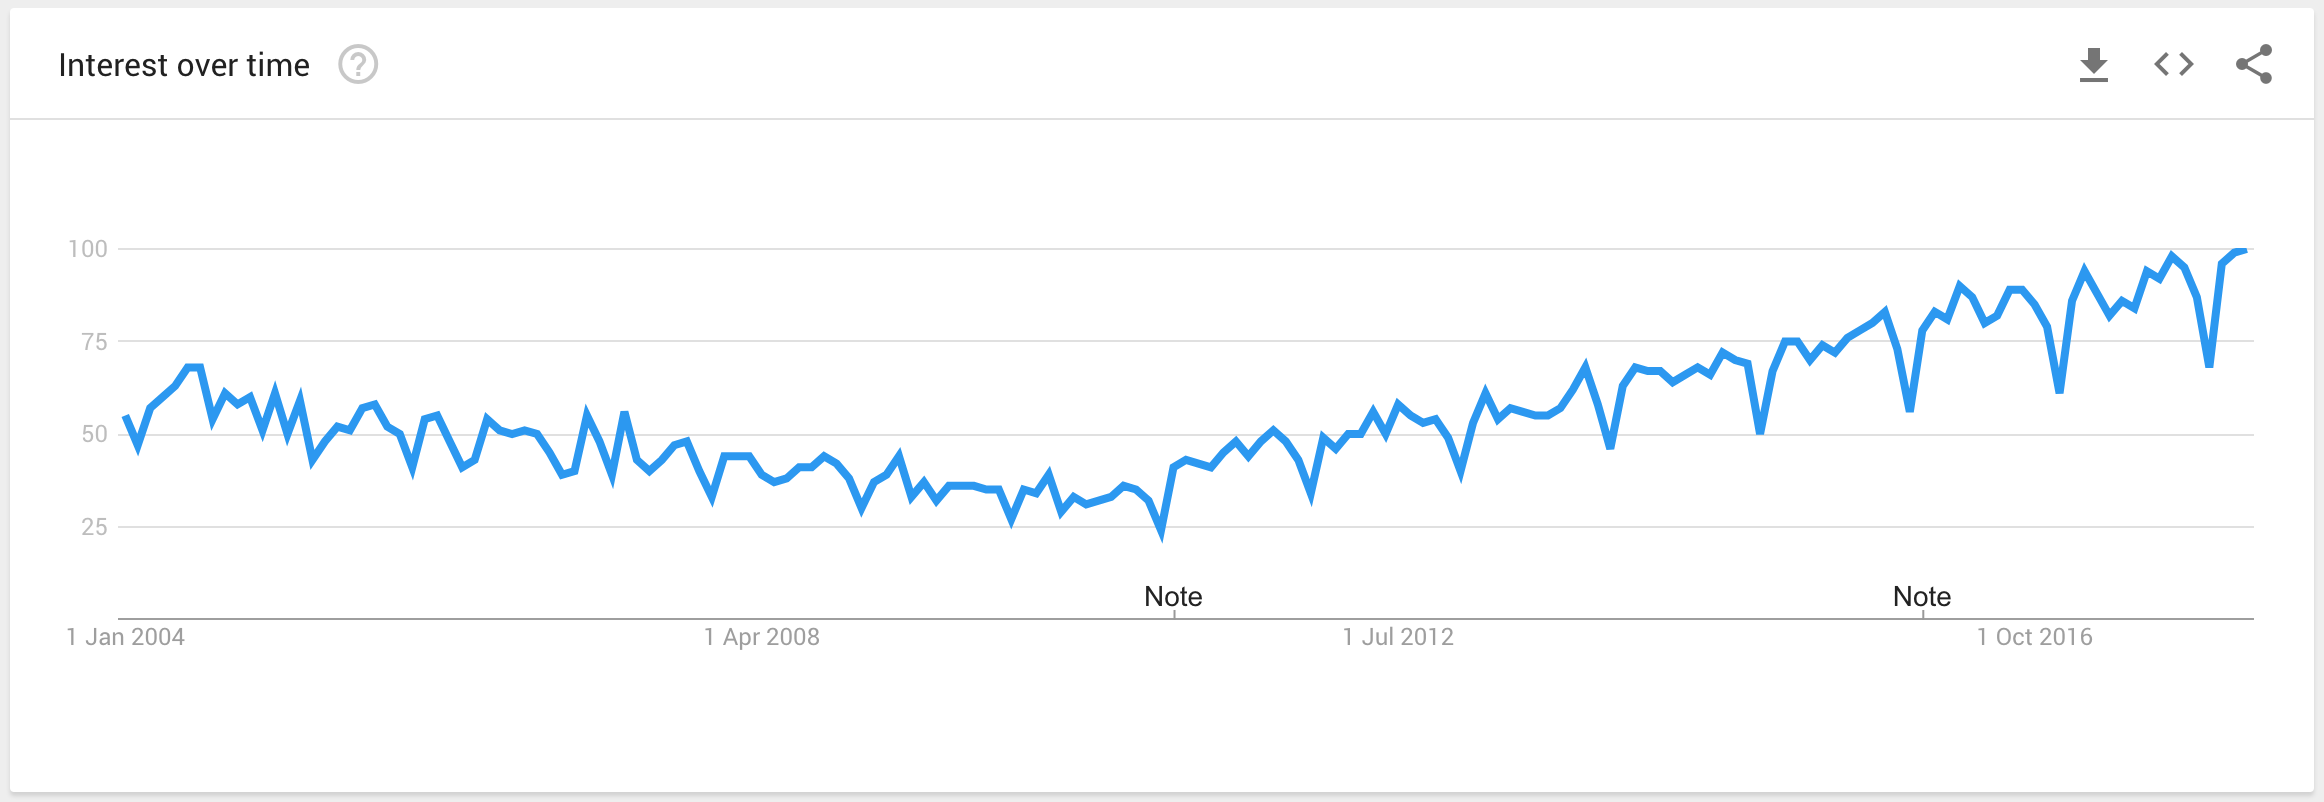
\includegraphics[width=\textwidth]{birthday_cards_google_trends.png}
    \caption{Google Trends result for 'Birthday Card' from 2004 - present in the United Kingdom}
    \label{fig:google_trends}
  \end{figure}

Google Trends allows us to see the most recent information on the interest a market. From this, it is evident that interest in greetings cards in the UK continued to increase throughout 2017 and into 2018. There are no signs that this increase is slowing, and as a result there is plenty of space in the market for new innovations that increase the accessibility of cards to consumers.

This growth is unsurprising, as the UK is already a significant part of the global greeting cards market. The UK market is the largest in Europe \citep{strategyr}, and sells more cards per capita than anywhere else, at 33 cards per person per year \citep{greetingcardassociation}. It is suggested that this is because sending and receiving cards is an important part of culture in the UK \citep{greetingcardassociation}.

The biggest area of competition for this product will be online; the decline of the greetings card industry elsewhere is attributed to the ease of sending a greetings message over the internet \citep{npr}. While this is noted as a threat to the UK industry, it has not had as large an impact as it has in other countries\citep{mintel}. Our goal is to introduce a service that is equally easy as sending a message online, but also retains the meaning and thoughtfulness behind traditional card giving.

There have been multiple startups, especially in the United States, that focus on the meaningfulness aspect. For example, Lovepop, a manufacturer of three dimensional pop-up cards received financial backing on the TV show Shark Tank \citep{americaninno} and has since seen success from selling their high-end cards through Etsy \citep{Etsy}. It is premium cards similar to these that we plan to use as they are more special and unexpected.

In the UK, a notable startup is Moonpig, an online service that delivers personalised cards directly to the recipient. They have continued to grow since their \pounds120m acquisition by PhotoBox \citep{bbc}. While Moonpig and its competitor Funky Pigeon are successful, market research still suggests that online card sales are lagging behind sales from physical stores \citep{mintel}, meaning there is room for innovation in this area.

\subsection*{Primary Research}
We wanted to get feedback on our idea early on, before we had invested too much time and effort into it, but struggled to find any experts in the greetings card industry. Instead, we focussed on approaching people who may want to use our service, and people who may be likely to receive cards delivered through our service. We decided to interview a range of these people rather than using questionnaires; interviews enabled us to get a more detailed and personal exploration of the interviewee's needs, as we could ask them to elaborate if we didn't understand anything they said, or probe for more information.

Before asking individuals specifically about our service, we firstly asked them more general questions in order to gain a firmer understanding about how they send greetings cards and how they feel about receiving them. This enabled us to refine our business idea based on their feedback, before carrying out a second round of interviews focussed on finding their thoughts about our refined idea.

For the first round of interviews, we used a set list of questions which consisted of the important questions that we had discovered from part A, and also from analysing the user needs we had previously ascertained. We interviewed a total of eight people, and conducted the majority of the interviews in person. Some of the interviewees were students, and some were working adults. The full interview results are included in the appendix, and some relevant key findings are listed below:
\begin{itemize}
  \item There was a mixed response on whether or not people struggle to remember to send greeting cards
  \item Nearly everyone said that they remember birthdays and important dates without the aid of any physical or virtual tools
  \item Five out of eight of the interviewees said that the quality of a card is important
  \item The majority of interviewees preferred to receive a card with a handwritten message inside, rather than a personalised, printed one
\end{itemize}
The first and second points consolidate our hypothesis that an automated card sending service may be useful for some people, but not so much for others. Upon hearing that five of the eight interviewees felt that the quality of a card is important, we decided to focus our service on luxury greetings cards, rather than budget ones. Originally we had thought that the service could print the message inside the card in a cursive font and send it directly to the recipient, but after hearing that people generally preferred to receive a handwritten card than a printed personalised message, we chose to not include that feature. We now envision that a blank card will be sent to the customer along with the envelope complete with the recipient's address and a prepaid stamp, so that they can write their message inside the card and mail it to the recipient.

Next, we created some new interview questions designed to find out how people felt about our newly refined business idea. We interviewed three people who had previously mentioned that they find it hard to remember to send cards and care about the quality of cards, as this would be our target audience. Again, the interviewees were a mixture of students and working adults. Full results are in the appendix and below are some key findings:
\begin{itemize}
  \item People expressed interest in the idea of an automated card sending service
  \item People expressed interest in the idea of receiving an envelope with the recipient's address and a prepaid stamp and a card which they can hand write and send themselves, presumably as this wouldn't be too much effort and would be more personal
  \item One interviewee mentioned that they would like to be able to choose the category of card to be sent
\end{itemize}

The results are positive and suggest that our idea has potential, however we are aware that we may be a victim of the ``Mom Test''. To combat this, we asked questions such as ``would you prefer a system which offers x or y'', rather than ``how do you feel about a system offering x''. This did make it harder to gain results specifically about our business idea, and we are also aware that the results we did find may have been influenced by a social bias, as we had interviewed friends and family.

Therefore, for to gain further and more concise market validation, we have planned to create and launch a prototype website where customers can sign up to our service, and analyse it to discover whether there is in fact a market for our idea. If we were properly launching our business, we would need a partner greetings cards firm to create the cards for us and send them to the customers. However, we want to find out whether people would use our system before investing too much time into it. Therefore we plan to manually buy and send the cards to customers ourselves. This will be the next step we are planning to take.

\subsection*{Competitors}
Our main competitors fall into three categories. Firstly, there are the card shops or supermarkets selling greeting cards, such as Sainsbury's and CardFactory. We aim to differentiate our business firstly by offering convenience --- customers do not have to go to a shop to buy a card. Secondly, our service is automated, meaning that customers do not have to actively try to remember their contacts' meaningful dates. Customers enter the dates into Natalis and are notified by email when the date is draws near.  Finally, our service will offer high end greetings cards, whereas these shops generally offer cards towards the lower end of the market. Although these companies are successful, these differences should ensure that our company will not be in direct competition with them.

The next group of competitors we will face are online greetings card companies, such as MoonPig and Funky Pigeon. These businesses are well established within the market, therefore it is imperative that our value proposition differentiates Natalis from these incumbents..
Again, we will differentiate ourselves by providing an automated card sending service, and providing high end greeting cards. Specifically concerning these competitors, our service is unique in how the personal aspect of sending cards is maintained. Customers may still write the message inside the card, rather than having it printed by a computer, unlike the offerings of MoonPig and Funky Pigeon.

Finally, the last group of competitors will be e-commerce websites such as Etsy and Redbubble. These websites provide a platform for individual artists to sell a wide range of unique and handmade goods. We will differentiate ourselves from these competitors by focusing on the sale and distribution of handmade, quality greetings cards.

Table~\ref{table:competitor_analysis} directly compares the features of Natalis with the offerings of its competitors.

\begin{table}[h]\footnotesize\centering
 \begin{tabular}{ | p{2cm} | p{2cm} | p{2cm} | p{2cm} | p{2cm} | p{2cm} | }
    \hline
    Feature & Natalis & Supermarkets & CardFactory/ Clintons & Moonpig/ Funky Pigeon & Redbubble/ Etsy \\
    \hline
    Online & \cellcolor{tableGreen}Yes & \cellcolor{tableRed}No & \cellcolor{tableRed}No & \cellcolor{tableGreen}Yes & \cellcolor{tableGreen}Yes \\
    Card Specialist & \cellcolor{tableGreen}Yes & \cellcolor{tableRed}No & \cellcolor{tableGreen}Yes & \cellcolor{tableGreen}Yes & \cellcolor{tableRed}No \\
    Premium Cards& \cellcolor{tableGreen}Yes & \cellcolor{tableRed}No & \cellcolor{tableRed}No & \cellcolor{tableRed}No & \cellcolor{tableGreen}Yes \\
    Reminders & \cellcolor{tableGreen}Yes	& \cellcolor{tableRed}No & \cellcolor{tableRed}No & \cellcolor{tableRed}No & \cellcolor{tableRed}No \\
    \hline
  \end{tabular}
  \caption{Feature comparison between Natalis and its competitors.}
	\label{table:competitor_analysis}
\end{table}

\section*{Strategy}
\subsection*{Legal Status and Business Structure}

As an online retailer, there are laws we must abide by regarding what information we make clear to customers on our website (e.g. terms and conditions, contact details). These will be thoroughly investigated as part of the website design stage to ensure compliance. We must also consider data protection laws, because is inevitable that we will require some personal information from our customers. Payments will be processed using a third party payment provider (see section \ref{financing} for details), so we will not need to store any payment details. However, we will need to store personal information such as names and addresses. This means we must adhere to data protection regulations, as infringement of these would leave us liable to fines from the Information Commissioner's Office (ICO).

To ensure compliance with data protection regulations, a data protection impact assessment (DPIA) should be carried out to identify potential security concerns with how data is stored. This is mandatory for compliance with the EU General Data Protectection Regulation (GDPR), which will be enforced from 25th May 2018. The ICO also recommend tasking one member of the team with responsibility for day-to-day security measures. This includes responding to data protection requests within 40 days, and periodic checks to ensure the organisation's security measures remain appropriate and up to date. An example of a security measure that should be taken is encryption of user data stored in SQL databases. Furthermore, under data protection law, we will need to notify the ICO of how our organisation handles personal data about our customers.

The business structure we have opted to use is a limited liability company (LLC). Unlike a partnership, this means the company is a separate legal entity to the company directors. This reduces our exposure to financial risk, as if the company were to go under (for example, if our data protection measures were insufficient and we were made to pay a fine we couldn't afford), the financial burden lies with the company rather than us as individuals. However, being an LLC comes with significantly more administrative and regulatory demands than a partnership. To become an LLC, we will need to register with the Companies House. As an LLC we will need to keep company records of our transactions and financial agreements, and file our accounts with the Companies House and our company tax return with HMRC. These accounting tasks will be assigned to a member of our team who will be responsible for their completion.

\subsection*{The Team}

\subsection*{Operational Plan}

\subsection*{Financing}

\subsection*{Sales and Marketing Plan}
Natalis will focus on relationship marketing to keep customers engaged and increase their customer lifetime value.

\subsubsection*{Direct Touchpoints}
\paragraph*{Email}
Email is the primary method which we will use to keep in touch with existing customers. In addition to the reminder email sent to the customers in advance of their contact's important date, we will keep in contact with customers through a number of marketing strategies.
\begin{enumerate}
	\item Email Newsletter: An email newsletter will be used to keep customers up-to-date with new card styles, card artists and potential future product launches, as the company grows. Furthermore, this email newsletter will inform consumers who registered in advance of the product launch when Natalis launches and will prompt them to sign up.
	\item Promotional Newsletter: We will offer promotions to customers through emails to increase sales. Seasonal promotions will be a particularly useful strategy if run around popular holidays, like Christmas, when people are likely to send many cards. An example offer could be: ``Send 5 cards and get 1 free!''. In addition to increasing sales, by persuading customers to reach the minimum order size required for a free card, they will become more accustomed to using Natalis and ultimately more reliant, encouraging them to return.
\end{enumerate}

\paragraph*{Social Media}
Social media will be our primary platform used to reach new customers. We propose to exist on all popular social media channels including Twitter, Facebook, Snapchat and YouTube. Having a presence on multiple channels increases our reach and as content can be posted on multiple sites, does not add cost for each new site we have a presence on. Despite the ability to share content across multiple networks, we will tweak it to play upon the strengths of each site by tailoring the style of content to drive consumer engagement. For example, Twitter marketing works best when the updates we provide are brief and impactful with a short information half-life. Likewise, YouTube can be used to launch a video advertising campaign. Ideally, this campaign will spur organic growth in the customer base when they are shared by consumers to their own social feeds and are given greater exposure.

We will also use social media for targeted advertising to raise awareness of Natalis to potential customers. Social platforms, enable advertisers to reach consumers in specific demographics based on information collected on them through their social network and browsing activity. Through this means, we will be able to run an advertisement campaign targeted at our target audience. The advertisement campaign will mirror the anecdotal messages we display on the website.

\paragraph*{The Natalis Website}
The Natalis Website is where consumers will convert to customers. The website will convey the Natalis subscription to consumers and emphasise the needs we aim to solve with practical and anecdotal messages which will help the consumer understand why they want to use Natalis. For example, we can display a user story where a father is surrounded by his children, all of whom are delighted that their Dad got them all loving, sentimental Christmas cards. We will also emphasise how fast and easy it is to subscribe to Natalis using messages such as ``It only takes 3 minutes to never forget again''. This way, user's will not be put off, by what they may falsely believe is an arduous sign-up process. The website will provide a link to subscribe to Natalis using the simple onboarding process and a link to manage the user's subscription.

\subsubsection*{Indirect Touchpoints}
\paragraph*{Social Media}
We will use social media as an indirect touchpoint by collaborating with digital content creators to promote our product. For example, we can provide Instagram influencers with a free subscription in exchange for a real endorsement of Natalis targeted towards their followers. We will aim to target influencers who have a following which overlaps with our target audience, and who have a large online presence (klout). The network coproduction model states that these influential users will help us to reach new customers through social channels. Typically, consumers are more likely to purchase a product if it is recommended by a community opinion-leader, therefore, by collaborating with these trusted content-creators, we are able to generate e-word-of-mouth marketing to promote organic subscriber growth. The relationships we form with content creators are beneficial for both parties: we gain exposure to more potential customers, and the influencer gains a free product and content to publish which their audience will have an interest in. However, we should consider the risk that this method of marketing, if not transparent, it can damage the reputation of our brand and of the influencer.


\paragraph{SEO and SEM}
We will use Search Engine Optimisation (SEO) and Search Engine Marketing (SEM) techniques to appear more highly in search engine results. We will focus on raising our search engine ranking for search terms associated with \textit{greetings cards}, \textit{greetings card delivery services} and \textit{handmade greetings cards}. More specifically, we will focus our SEM towards terms like \textit{Birthday}, \textit{Christmas} and \textit{Anniversary} which consumers are more likely to search for than greetings cards. However, as our product is unique in the small online greetings card market, we expect to appear near the top of search results without the need for SEM. Together, these techniques will help us to reach consumers beyond our direct touchpoints.

\subsubsection*{Sales and Marketing Costs}
The costs of marketing have been estimated in our income statement found in Appendix \ref{app:income_statement}. The estimated marketing costs are based on the two main marketing strategies that we plan to use: online advertising and promotional videos. It is assumed that the cost to operate social media and email touchpoints will be negligible. The cost of online advertising was calculated using estimates from research performed by WordStream \citep{wordstream} into the cost of Facebook advertising, although SEO and SEM will share a proportion these costs. The cost of promotional videos was based on the cost to hire actors only. Other costs such as filming, editing and set design could be provided by the Natalis team at no cost as we have sufficient equipment and experience in this domain. A fair rate of pay for the performing actors was quoted by The Casting Network \citep{casting}. The videos will involve six actors and be updated every two years.

We will only make sales through the Natalis website. This website will be free to create, as the team possess all of the necessary development skills required to build and operate the site. The operational costs of the website are listed in the income statement under the heading: \textit{Website Development / Management}. The Cost of Goods Sold (CoGS) is explained in the Financial Data section of this business plan. There are no other sales costs associated with Natalis.


\section*{Risk Analysis}
\subsection*{Product Risks}
Insufficient Selection of Card Designs: Having a choice of card designs to choose from is most strongly associated with the functional values which drive consumer choice. An insufficient choice of designs for the consumer will mean their functional needs may not be fulfilled beyond what our competitors can offer. Furthermore, a poor selection of designs can lead to the non fulfilment of social values in the case where the cards do not portray the social image of the consumer. Lastly, if the offered designs cause a negative emotional response in the recipient, it is unlikely that the emotional and belonging needs of the consumer will be fulfilled. The fulfilment of all needs is key to getting customers to join our service.

\subsection*{Industry Risks}
As in any industry with competition, there are a number of risks involved. One of the largest risks of any startup is lack of demand. Given that the card market is already well-served, we are counting on our unique selling point to win customers. However, this carries the risk that these customers will not value our selling points highly enough to warrant changing their habits to involve a subscription service. To mitigate this, it may be necessary to advertise directly to our target audience.

Another risk is that, given the low entry barrier to starting our business, it would be trivial for a company with more advertising resources (such as Hallmark) to duplicate our service. This is compounded by the fact that our idea is too simple to protect through legal devices like patents. To mitigate this, we aim to target a section of the market which is currently underserved by the majority of the established companies---even if Hallmark were to duplicate our service, they'd still be selling Hallmark cards rather than handmade ones, thus appealing to different audiences.

In order to supply through Etsy's or Redbubble's wholesale scheme, we need to submit an application giving details about our business. There is a risk that this application could be rejected, in which case we would need to consider other supply options. We should take great care to make our application as strong as possible to try and avoid this situation, perhaps by having a completed website before making the application so we have something tangible to show them. There is also the risk that these companies change their terms of service once we are somewhat reliant on them, e.g.\ taking a bigger cut from the sellers and allowing them to sell at a higher wholesale rate in return.

\subsection*{Market Validation Risks}
Research conducted during market validation found that while the greetings card industry is growing in the UK, it is declining globally due to competition with online social websites. A potential risk to our service is an unexpected eventual decline in the UK market making it more difficult for us to compete. This can be mitigated by setting ourselves apart from the competition by targeting a higher end audience and marketing the service to focus on the meaning behind sending the card.








\bibliographystyle{bath}
\bibliography{refs}
\clearpage

\begin{appendices}
\section{First Round Interviews}
\label{sec:firstRoundInterviews}
\begin{landscape}




  \begin{figure}
  \vspace*{-2cm}
  \makebox[\linewidth]{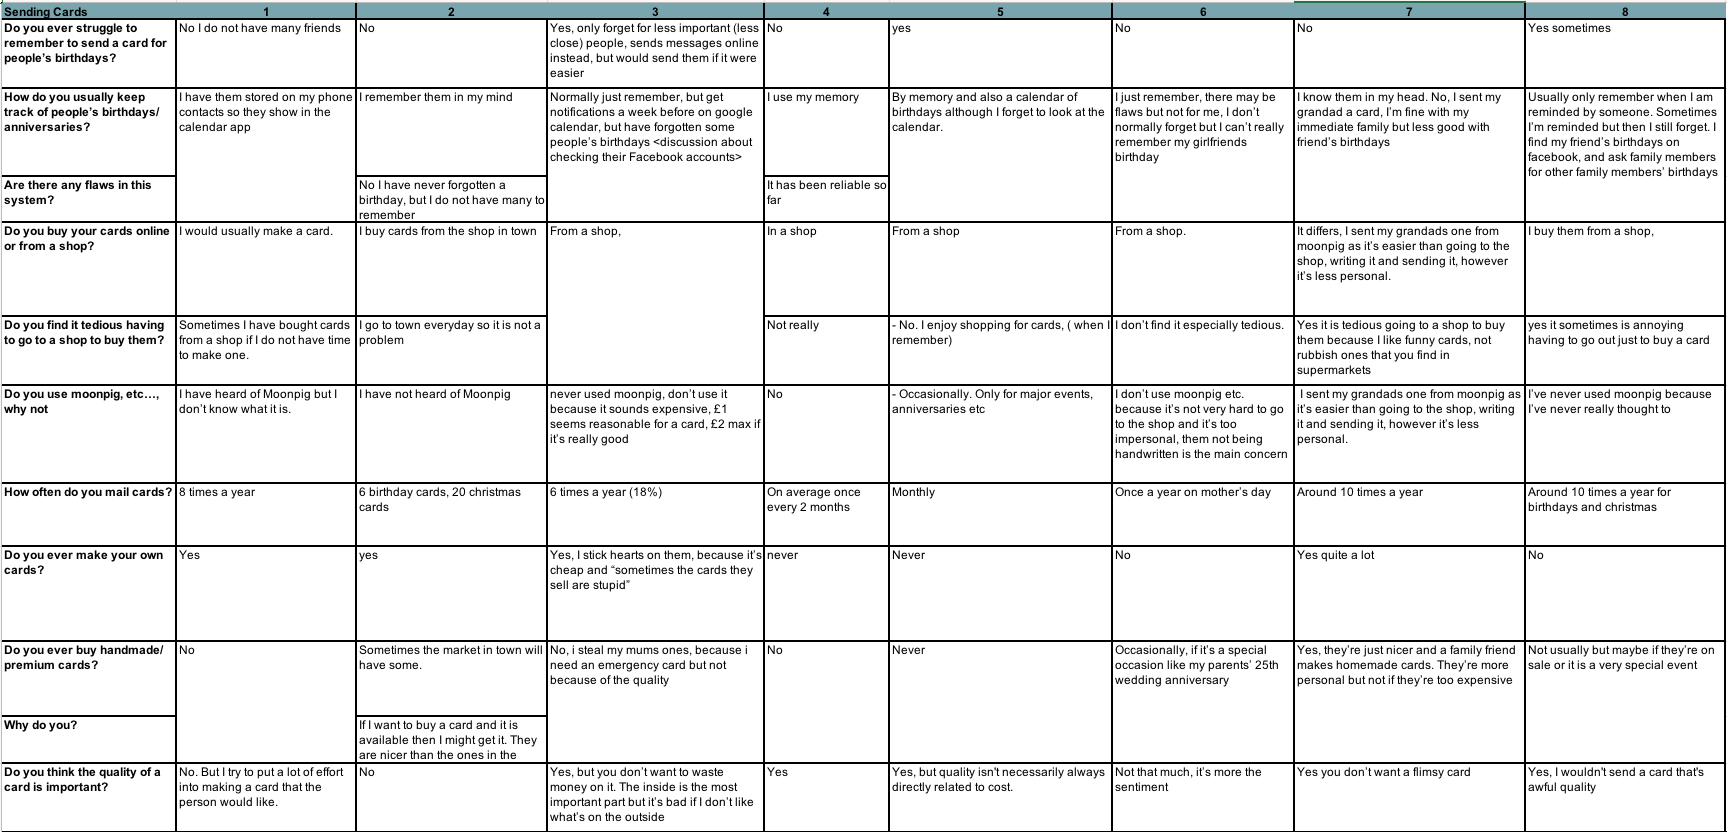
\includegraphics[width=1.0\linewidth]{primary_research_1.png}}
    \caption{First Round Consumer Interview Results -- Part 1}
  \end{figure}

\clearpage


  \begin{figure}
  \vspace*{-2cm}
  \makebox[\linewidth]{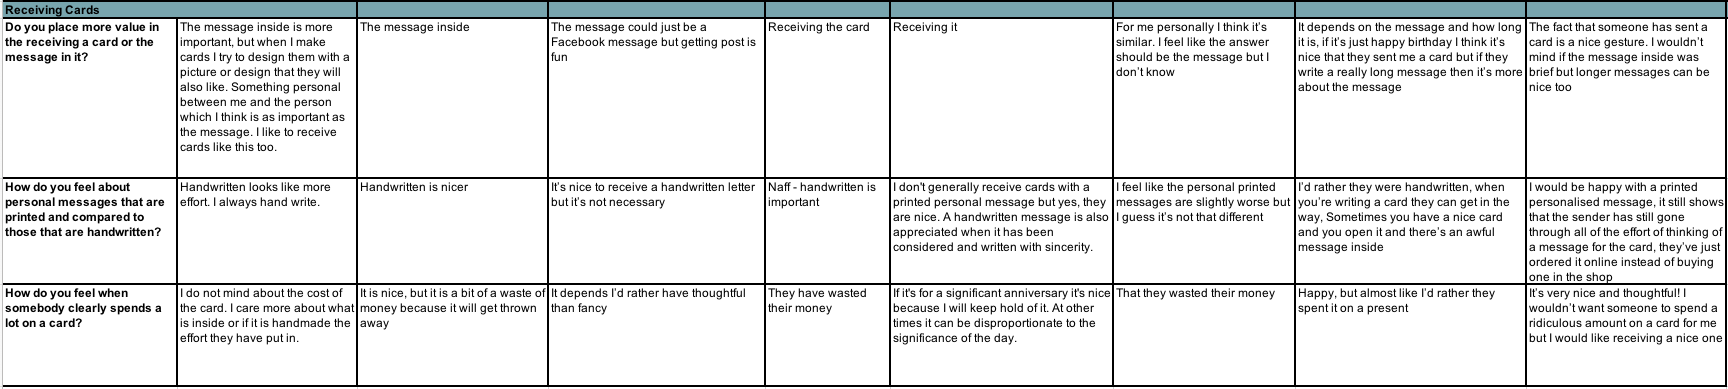
\includegraphics[width=1.0\linewidth]{primary_research_2.png}}
    \caption{First Round Consumer Interview Results -- Part 2}
  \end{figure}
\end{landscape}
\clearpage

\section{Second Round Interviews}
\label{sec:secondRoundInterviews}


  \begin{figure}[!htb]
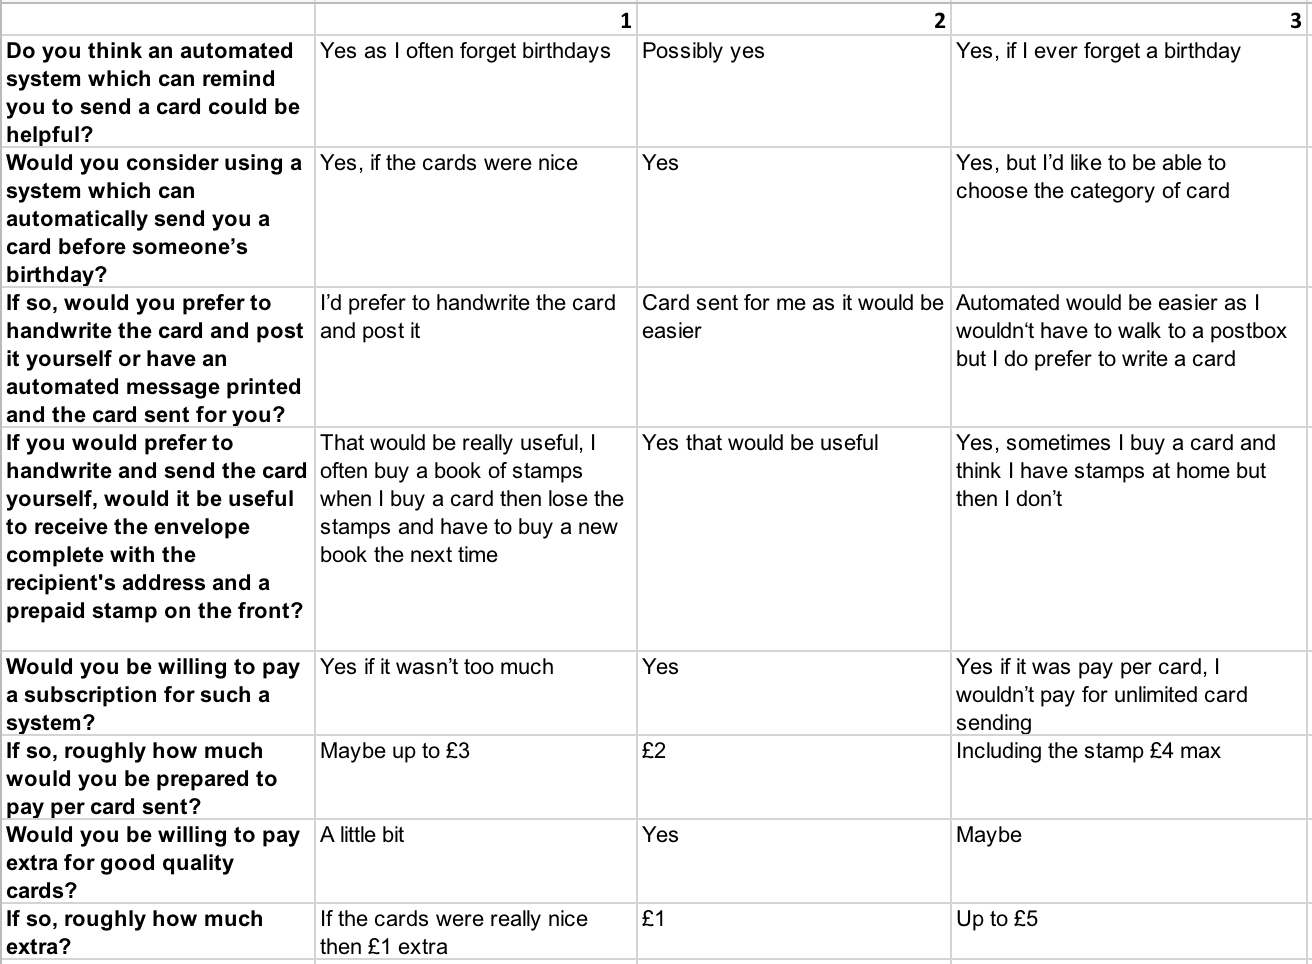
\includegraphics[width=1.0\linewidth]{primary_research_3.png}
    \caption{Second Round Consumer Interview Results}
  \end{figure}



\clearpage
\section{Income Statement}
\label{app:income_statement}
  \begin{figure}[!htb]
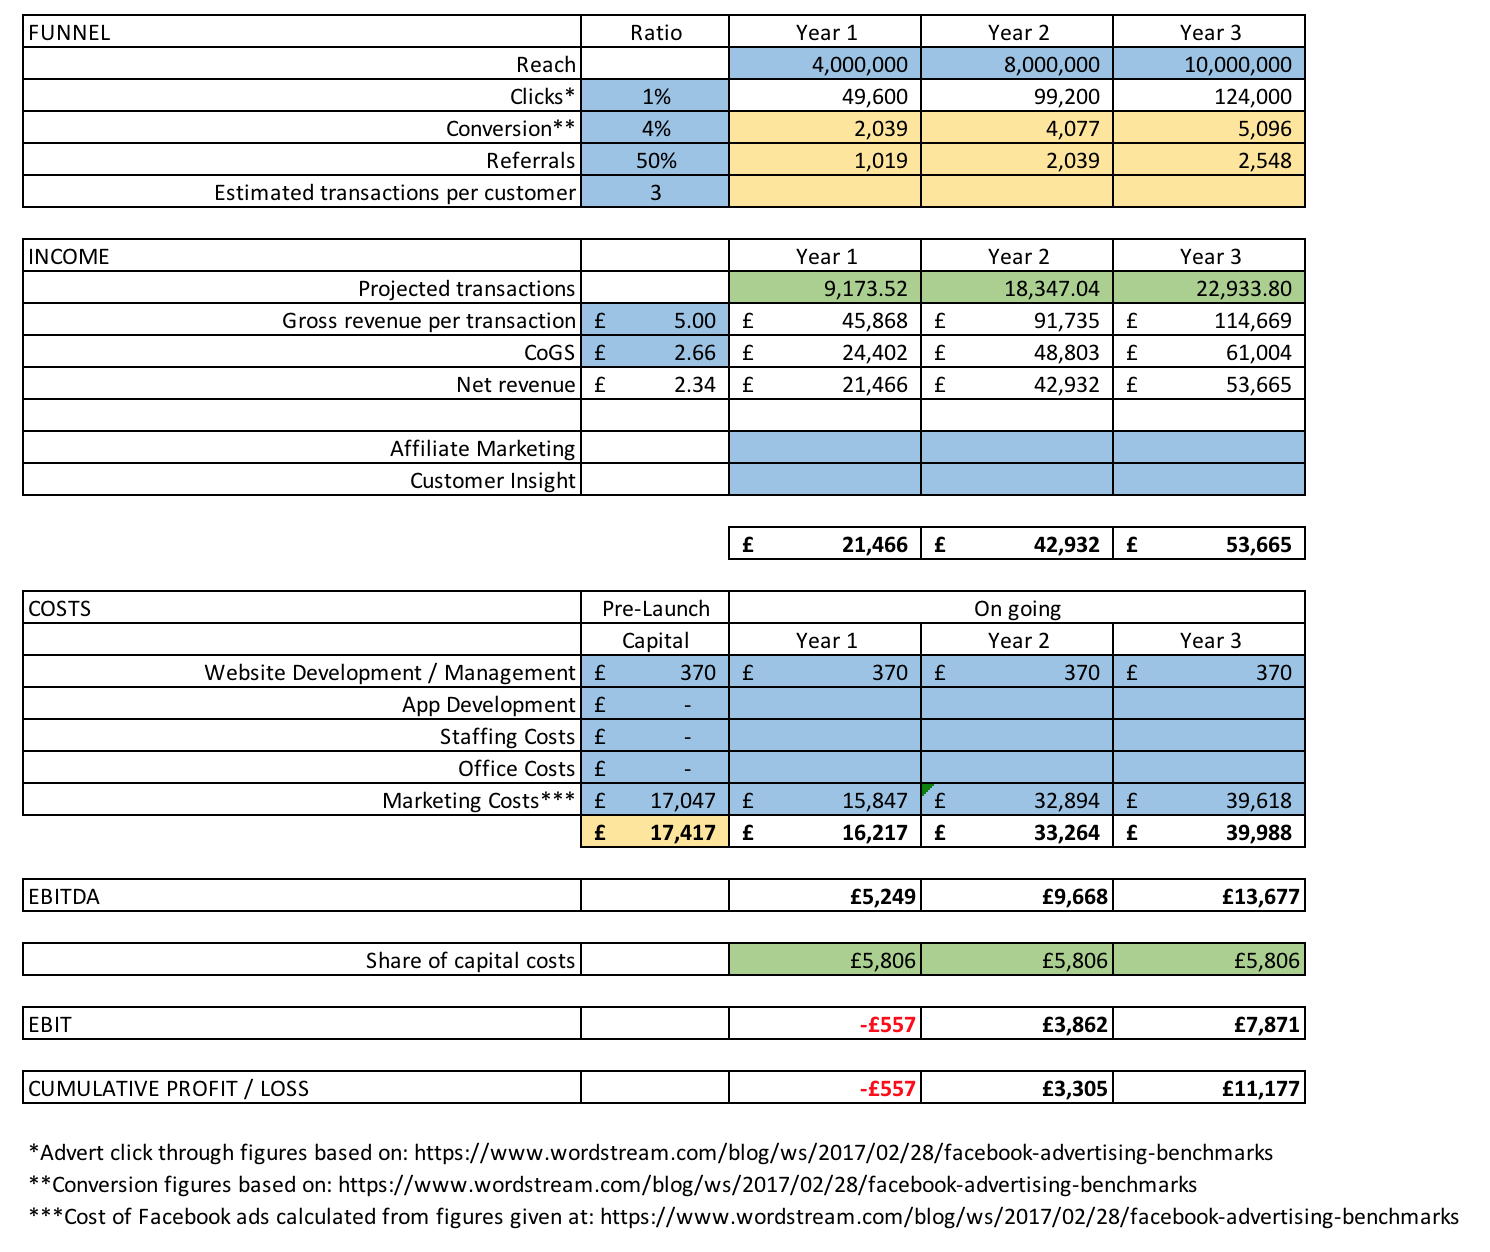
\includegraphics[width=1.0\linewidth]{income_statement.png}
    \caption{Natalis projected income statement.}
  \end{figure}


\clearpage
\section{Individual Contributions}\label{sec:individualContributions}
\subsection{William Kennerley}\label{subsec:williamKennerley}

My most important individual contribution to the first coursework was in the first section, \textit{Our Product}. In this section I introduced the problem we are trying to solve, the consumer needs, described the alternatives which we considered, helped to write the value proposition and discussed the risks we recognised as part of the risk analysis. In addition to this, I wrote the cover sheet elevator pitch, I gave guidance to the team based on my previous experience writing a business plan and made suggestions across the document when proof reading.

There were two major problem areas which I faced:
\begin{enumerate}
  \item Determining consumer needs
  \item Narrowing down alternatives to construct a focused value proposition
\end{enumerate}
In response to the challenge of determining consumer needs, I read the academic source material for the following key theories on human motivation and consumer values:
\begin{itemize}
  \item Maslow's Hierarchy of Needs
  \item McClelland's Human Motivation Theory
  \item Herzberg's Two Factor Theory
  \item Deci and Ryan's Self-Determination Theory
  \item Sheth, Newman and Gross' Theory of Consumption Values
\end{itemize}

I had to choose which of these theories was most appropriate to determine the needs of our customers. I first ruled out using McClelland's Human Motivation Theory and Herzberg's Two Factor theory as they focus on motivation within organisations and they do not address why people buy products. Likewise, I ruled Deci and Ryan's Self-Determination Theory as the most influential conclusion of this theory, intrinsic motivation, could be implied when discussing the social value \citep{sheth1991we} which greetings cards provide.

I chose to use Maslow's Hierarchy of Needs for its fundamental importance in psychology and its usefulness in identifying the basic needs which our product would fulfil. Recognizing the consumer needs was essential, as it let us determine if any competitors already met all the needs of our target market. If a competitor did match all the needs of our target market, we would need to restructure our VP or pivot. I also chose to use the Theory of Consumption Values by Sheth, Newman and Gross as it could be used to accurately pinpoint why consumers would want to buy our product and not our competitors. By identifying why consumers choose to purchase products and more specifically, greetings cards, we could design Natalis to be the most appealing player in the market.

After determining the needs of the consumer and their consumption values, narrowing down the features (alternatives) of our product to form a value proposition was straightforward. To do this, I listed all the proposed features along with the consumer need or value they fulfilled. Where a need or value was fulfilled by two features of the product, one of the features was planned for removal. To confirm the choice of which features to remove, we conducted primary research with potential users. I contributed to the primary research by holding some interviews. Through this process, I could help to construct a focused value proposition.

In the second coursework I revised the needs and value proposition based on the feedback we received. I also created the marketing plan by choosing between alternative touchpoints we could use to reach consumers. This involved researching the costs of each marketing strategy which were subsequently added to the financial statement. 

\clearpage


\subsection{Ben Plumley}\label{subsec:benPlumley}
 The most important individual contribution I made to the coursework was the research and writeup of our competitors and suppliers. This made up around half of the Industry Analysis section, and part of the Risk Analysis section.

This involved researching the business models and supply chains of the following companies:

\begin{itemize}
	\item Hallmark
	\item Clinton
	\item Card Factory
	\item Cards Galore
	\item Sainsbury's
	\item Tesco
	\item Archway Cards
	\item numerous independent shops
\end{itemize}

Problems encountered while researching this section included the fact that shops are unlikely to provide information about their supply chain, possibly to maintain a competitive advantage. However, by analysing the portfolios of larger suppliers, I was able to infer which shops were supplied by which companies.

This allowed me to make like-with-like comparisons between shops using the same suppliers, and will also help us to cut out extraneous middlemen and resellers when finding our own suppliers.

Once I had an accurate idea of the current competitive landscape, I was able to look further into the portfolios and strengths of each supplier to determine which would be appropriate for us to develop a relationship with. This also ties strongly into the latter half of the Industry Analysis section.

My findings showed that while the businesses I'd analysed could supply cards to us, they would only be able to supply the lowest-end cards we offer, due to the way the target markets overlap. This informed research into the hand-made and artisan markets which would make up the remainder of our suppliers.

Additionally, I proofread and offered suggestions and improvements on all other sections of the document.

\clearpage
\subsection{Max Sandberg}\label{subsec:maxSandberg}
My most important role in the creation of the business plan was having joint responsibility for the Industry Analysis section. Once we had all agreed on the business we wanted to make and how it would work, we delegated different sections of the business plan to different members of the group. As there are 6 group members, we assigned 2 people to each of the first 3 sections, and agreed that each pair would also write the part of section 4 that was relevant to their section. The two of us then formed a list of all the companies we wanted to discuss in this section, and split this list between us. I was left with the following list of companies to research and consider our relationship with:

\begin{itemize}
	\item Moonpig
	\item Funky Pigeon
	\item Etsy
	\item Redbubble
	\item M\&S
	\item John Lewis
	\item Facebook
	\item Whatsapp
\end{itemize}

Once we had all written our sections, we compiled them into a single document. I feel that this approach was a fair and effective way of splitting the workload across the group. I also proofread and made suggestions on the rest of the document, then implemented the suggestions others had made for the parts that I wrote. I believe this lead to a significant improvement in the overall quality of the business plan.

One particular development in our business strategy came about as part of my research into e-commerce businesses such as Etsy and Redbubble. Our understanding of these websites previously came only from our previous experience using these websites as consumers. This meant that when we discussed using sellers from these websites as our suppliers, we imagined this sales process to be much like the process of buying cards from these sellers as an individual consumer. It was only when looking into their terms of service that I discovered these sites have an entirely different scheme, designed for businesses to buy from the sellers at wholesale prices.

This was an interesting development, particularly due to the wholesale prices of these cards being at least half that of the normal retail prices. This is a significant saving over the prices we had expected to be paying, and therefore a big improvement to the potential profitability of the business. I discussed these findings with the team, and we decided that buying our supplies through one of these wholesale schemes would be a good decision. I then went back and made the appropriate changes to the business plan to reflect this change.
\clearpage
\subsection{Oliver Gray}\label{subsec:oliverGray}
My primary focus was on market validation. I was involved in the creation and refinement of the original interview question set, and conducted six interviews with potential users and recipients. In addition to this I carried out the secondary market research. As result, it followed that I would work on the ``Market Validation'' section of the report, in particular the ``Importation Questions'' and ``Secondary Research'' subsections.

A key decision was on what questions to ask the interview participants. For this I took the ideas that were found during brainstorming and from the consumer needs analysis, and conducted some interviews using those ideas. This process strengthened some of the original ideas we had, and also allowed us to discard some others that we found were unpopular with the initial interviewees.

In addition to this, my role was to determine the current state of the market, so that we could show there was space for us to operate within it. This would clearly require research. I faced few problems finding useful secondary information as there are many greetings card associations and market research reports with statistics that are easily available.

The only barrier to the research was that only a summary of the report was available without paying a substantial amount of money (typically \textsterling750-2000). However, I think that a summary of the information is acceptable at this stage as we are only interested in finding out if there is a market for our idea, as opposed to optimising our performance within that market.

\clearpage
\subsection{Caroline Moir}\label{subsec:carolineMoir}
My main contributions to the coursework were interviewing people to acquire information for our idea, analysing their feedback and exploring which factors differentiate our idea from our competitors. In the final business plan, I also explored the roles of each of the team members, and how the areas in which we are each skilled in help to produce an effective help. Ollie made the questions for our first interview and then him, me and Will each interviewed people with them. I then analysed this feedback, created a second interview template, and used it to further interview some more people. I also assessed our main competitors, and explored the defining features of our idea which would differentiate us from them.

Therefore the part of the coursework most affected by my contributions was the market validation section in component 3, more specifically parts C and D of it, and also component 4b.

One of the problems I faced was the struggle of finding a wide range of people to interview. I wanted to ensure that I got a broad range of opinions and did not only interview one group of people, i.e.\ students, as these were the group of people who were easiest for me to talk to. Also, another problem I experienced when conducting interviews was trying to ensure that we weren't affected by the ``mom test'' and social biases. The people I was interviewing may have been enthusiastic for any system I was proposing because they wanted to give me nice feedback, not because they actually would use the system.

I researched how to avoid our interviews being affected by the ``mom test'', and found that it was best to avoid asking questions specifically about our business idea and whether the interviewee would use it or not. Instead, a better idea was to ask them more generally about a scenario they have experienced and ask what problems they might have encountered during it.

To ensure that I was receiving varied opinions from different groups of people, I interviewed some people who I used to work with on placement, along with fellow students and family members. In order to not be a victim of the ``mom test'', I made interview questions such as ``have you ever experienced any problems when doing this'' and ``would you prefer x or y'' rather than ``would you use x''.

\clearpage
\subsection{Darien Opperman}\label{subsec:darienOpperman}
The contributions I made that had the largest impact on the project were my contributions to the "Our Product" section. Specifically, the \textit{Value Proposition} and \textit{Meeting Customer Needs} sub-sections. To complete these sections, a concrete, unified concept of the service had to be established within the group. Having a clear, well defined idea of the value proposition within the group allows for all other sections to be consistent.

As part of my effort to create a unified concept, I designed a series of logos, and edited them based on group feedback, going through multiple internal feedback stages.

The difficulties in clarifying the value proposition were due to subtle differences in perceptions and understanding. If one group member says the believe our business should be "classy", how do they interpret that word, and what implications does it have for our service? Lots of discussion within the group, and usage of other businesses as examples, were used to create an idea that I believe is now consistent within the group.

The differences in perception were highlighted in responses to logo design. Opinions on what an appropriate logo would look like varied within the group, with many members submitting suggestions and examples, some varying wildly, beyond simple differences in aesthetic taste. As a result, I researched logos, and the perception that consumers can generate based on a logo. This included research into existing popular logos, but also more abstract concepts such as emotional response to different colours.

My initial logo drafts relied too heavily on symbolic references to gift giving, sentiment, and warm social circle type feelings. Group response was negative due to this, and due to similarities between the imagery and charity company branding. Researching further, I found that symbolic references are not always required, and customers can create the sentimental links personally with any logo. Based on this, and more stages of group feedback, more logo drafts were devised, relying less on heavy symbolic meaning, and more on clean minimal branding that clearly indicated that greetings cards are the focus of the service.

On top of the above, my input also included some proofreading and small suggestions for other areas of the document.



\end{appendices}



\end{document}
